\chapter{Caso Concreto - IoT sensore Temperatura}
%correggere introduzione
Uno degli ambiti in cui viene maggiormente sfruttato Redis é quello IoT.
\paragraph{Cos'é l'IoT?\\}
L''Internet of Things é una tecnologia che permette di massimizzare le capacitá di raccolta e di utilizzo
dei dati da una moltitudine di sorgenti, le quali possono essere prodotti industriali, sistemi di fabbrica, veicoli
di trasporto e cosí via.
L'IoT consente di rendere disponibili i dati che servono a comprendere meglio il mondo reale.
Permette di estrarre informazioni utili ai processi decisionali.\\
Queste informazioni utili devono essere immagazzinate in maniera piú o meno persistente
e devono essere elaborate con dei tempi di latenza piuttosto brevi, ed é proprio qua che interviene Redis.

In questo capitolo verrá analizzata una possibile applicazione in ambito industriale, ma non solo:
verrá utilizzato un sensore di temperatura e umiditá che preleva delle informazioni ad intervalli regolari e
sfrutteremo Redis per la persistenza e l'organizzazione dei dati e l'elaborazione di essi.

\section{Arduino e DHT11}
Innanzitutto, il materiale necessario per questo progetto é:
\begin{itemize}
    \item Un microcontrollore compatibile con l'ambiente di sviluppo arduino e possibilmente con Wi-Fi integrato,
          nel nostro caso utilizziamo un ESP32.
    \item un sensore digitale di temperatura e umiditá dell'aria, utilizziamo un DHT11: costituito da una parte resistiva
    che si occupa della rilevazione dell'umiditá e da un NTC che rileva la temperatura, queste due parti sono gestite
    da un microcontrollore che é parte integrante del sensore.
\end{itemize}

Dopo che abbiamo collegato il tutto e verificato che il sensore funzioni correttamente, ovvero che mandi dei dati
coerenti all'ESP32 possiamo cominciare a sviluppare il progetto.

\paragraph{Sketch Arduino\\}
Dobbiamo sviluppare lo sketch che comunica con Redis Server e manda dati ad intervalli regolari.
Per fare questo vi é una libreria, chiamata \texttt{Redis.h} la quale permette di comunicare con il database Redis.
Eseguiamo una connessione sulla rete Locale sfruttando il modulo WiFi di ESP32.

Per fare questo prima di sviluppare lo sketch dobbiamo apportare dei cambiamenti al file di configurazione del server,
in quanto con la configurazione standard il server comunica solo su \texttt{localhost}(127.0.0.1).
Dobbiamo aggiungere un parametro per fare in modo che il server sia raggiungibile sulla rete locale aggiungendo indirizzo IP
privato della macchina sulla quale viene eseguito il processo \texttt{redis-server}.
Di conseguenza, il server sará raggiungibile tramite indirizzo IP e Port.\\
Nel nostro caso é: \textbf{192.168.179.25:6379}.
Dobbiamo anche aggiungere una password di sicurezza per l'autenticazione con il server, anche questo viene fatto
aggiungendo un parametro nel file di configurazione.

La configurazione viene modificata cosí:
\begin{lstlisting}[autogobble]
bind  127.0.0.1  192.168.178.25

requirepass "admin"\end{lstlisting}

 \\

Inizialmente dobbiamo sviluppare nello sketch la connessione con WiFi e, soprattutto, con il Server Redis.
Tutto questo avviene nel \texttt{setup()} perché deve essere eseguito solo all'accensione del nostro microcontrollore:
\begin{lstlisting}[autogobble]
#define WIFI_SSID "wifi-name"
#define WIFI_PSW "wifi-psw"
#define REDIS_ADDR "192.168.178.25"
#define REDIS_PORT 6379
#define REDIS_PASSWORD "admin"

WiFiClient RedisConn

void setup(){
    WiFi.mode(WIFI_STA);  //ESP32 associato come client alla rete WiFi
    WiFi.begin(WIFI_SSID, WIFI_PASSWORD);
    Serial.print("Connecting to the WiFi");
    while (WiFi.status() != WL_CONNECTED)
        delay(250);

    if (!redisConn.connect(REDIS_ADDR, REDIS_PORT))
    {
        Serial.println("Failed to connect to the Redis server!");
        return;
    }

    auto connRet = redis.authenticate(REDIS_PASSWORD);
    if (connRet == RedisSuccess)
    {
        Serial.println("Connected to the Redis server!");
    }
    else
    {
        Serial.printf("Failed to authenticate to the Redis server! Errno: %d\n", (int)connRet);
        return;
    }
}
\end{lstlisting}

Per quanto riguarda la connessione al Server Redis,  con \texttt{redisConn.connect(...)} creiamo una connessione con il server
passando indirizzo Ip e Porta che individuano il processo \texttt{redis-server}, successivamente proviamo ad autenticarci con
\texttt{redis.authenticate(...)}. Se tutto viene eseguito correttamente abbiamo il nostro \texttt{redis-client} che puó
comunicare.

Adesso bisogna passare all'invio dei dati al server: ovvero mandare i dati a Redis.
Per questo tipo di applicazione non si necessita di una fase di progettazione, in quanto
nell'ambito che stiamo discutendo abbiamo una mole di dati elevati ma semplici.
Nonostante ció, possono esserci diversi tipi di implementazione.
Ho individuato due modalitá, una per casi piú semplificati ed una per casi piú avanzati in cui si potrebbe disporre
anche di una rete di sensori.

Queste modalitá dipendono direttamente dalla struttura dati che intendiamo utilizzare in Redis per salvare i valori;
i due approcci in questione sono:
\begin{enumerate}
    \item metodo semplificato, dove ogni valore prelevato dal sensore lo memorizziamo in Redis con il tipo stringa,
          quindi avremo una tupla che viene generata per ogni prelevamento ad intervalli regolari, e sará cosí composta:\\
          key -> \textbf{nameSensor.time}\\
          value -> \textbf{sensor.value} \\
          Un esempio possibile quindi:\\
          sensorTemp.11:23:49 $\to$ 27.8
    \item metodo avanzato, dove viene utilizza una struttura piú complicata, non presente nelle strutture dati di base di Redis,
          chiamata \texttt{RedisTimeSeries}, é un modulo aggiuntivo che é stato fatto su misura per questo tipo di applicazioni.
          Permette un alto volume di inserimenti di valori con letture a bassa latenza. Puó essere vista come una SortedSet che associa
          ad ogni valore inserito un timestamp come score.\\
          Infatti sará fatto in questo modo:\\
          si crea una serie temporale il cui nome sará quello del sensore e all'interno della serie temporale verranno aggiunti i valori
          prelevati a intervalli temporali, e questi valori verranno associati al timestamp che corrisponde
          al momento in cui vengono inseriti.

     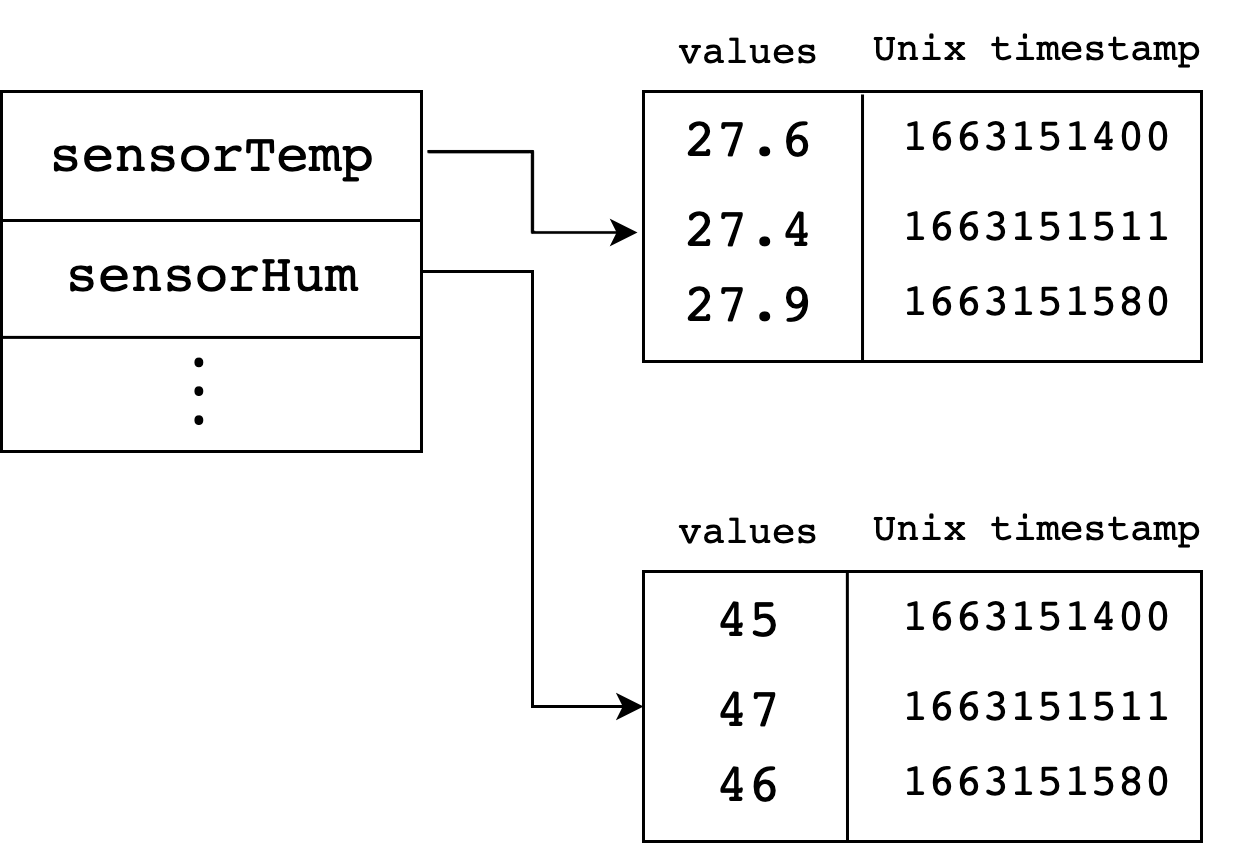
\includegraphics[width=0.7\textwidth]{img/redistimeseries}
\end{enumerate}






























%implementazione librerie Redis in linguaggi di programmazione
%Parlare di Jedis, libreria Java.\\


%Riportare esempi di codice che implementa DataBase.\\
%Descrivere progetto IoT fatto con sensore di temperatura DHT11.
%utilizzata scheda ESP32 che comunica con database e manda dati a redis server di rilevazione temperatura ogni 5 secondi.\\
%inserire parti di codice sketch arduino per far vedere come comunica con database.


%Illustrare software fatto con Java che preleva il dataset da redis server e lo elabora creando un grafico che si aggiorna in tempo reale.
